\chapter{Project Design} \label{chapter:model}

The design of the product will determine the user’s experience of using this software long before a result is shown. A prototype application was built during the first sprint that could take images display a result. This was made possible by the design page of Visual Studio MFC, to specify the interface between the application and the user. In an extensive UI design session during I prototyped different interface work-flows, sketching ideas onto paper windows frames. The user interface was simplified to minimise the options available to the user and we reduced each classification session to three views: Home Menu, SliderBar and Eulerian Dialog. An initial version of the updated design was completed by the end of June. 
\begin{figure}[!htb]
	\centering
	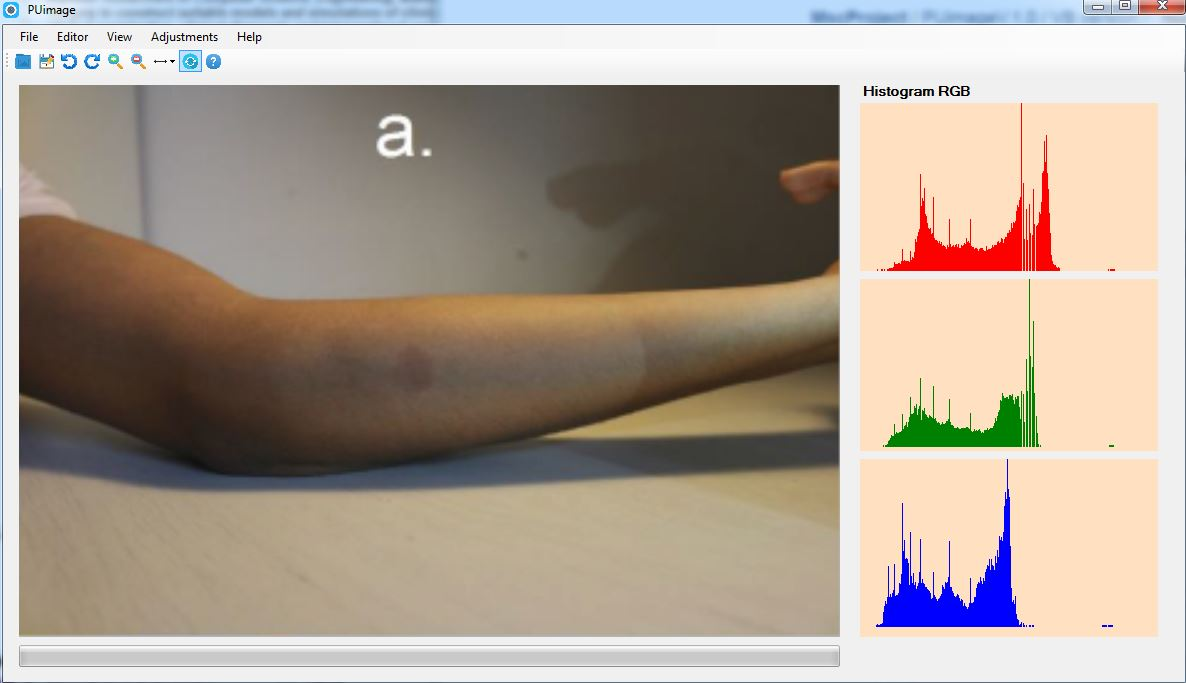
\includegraphics[scale=0.5]{img/originalProject}
	\caption{Original Software Design}
\end{figure}[H]

\begin{figure}[!ht]
	\centering
	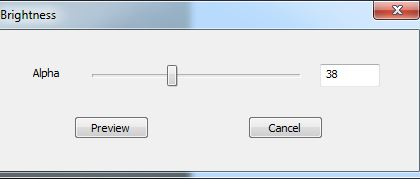
\includegraphics[scale=0.6]{img/brightdialog}
\end{figure}

\begin{figure}[!ht]
	\centering
	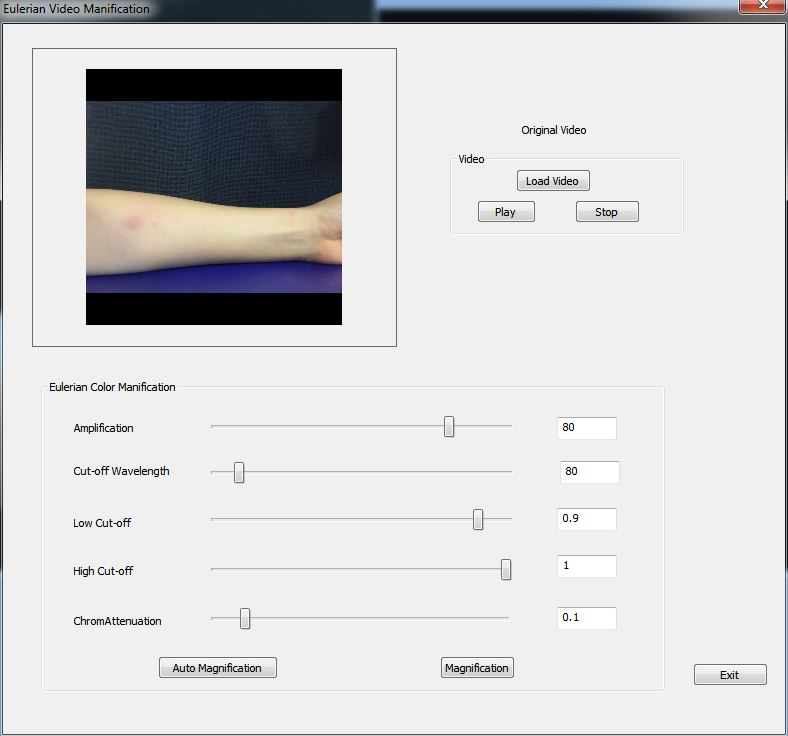
\includegraphics[scale=0.6]{img/eulerian}
\end{figure}

\begin{figure}[!ht]
	\centering
	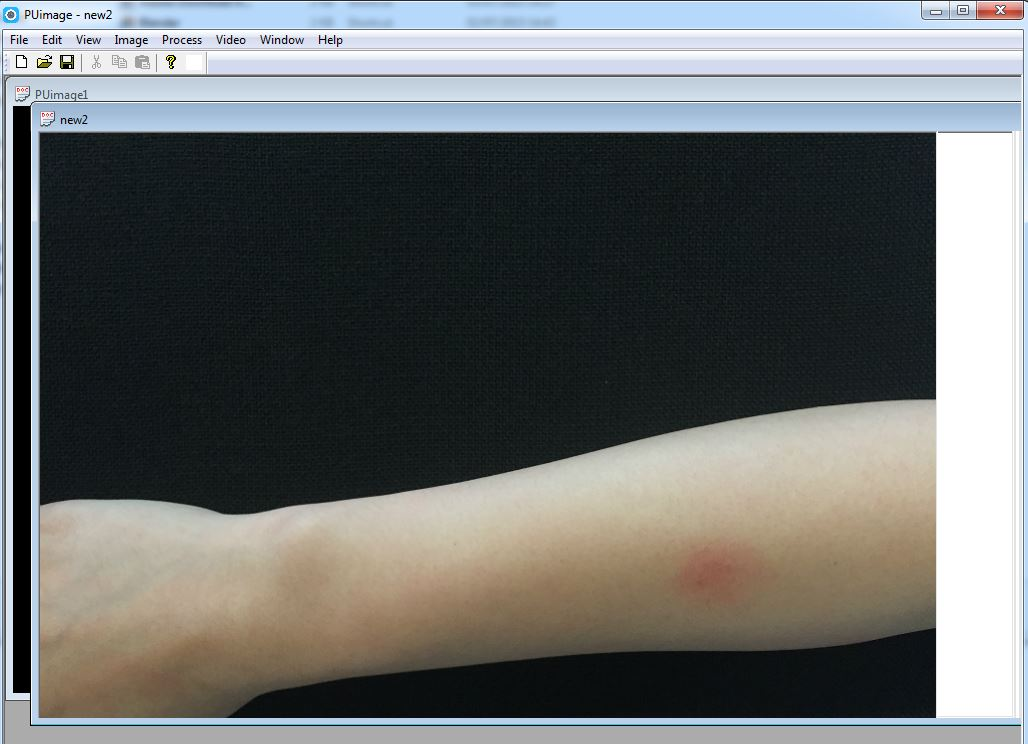
\includegraphics[scale=0.6]{img/nowProject}
	\caption{Latest Software Design}
\end{figure}